\begin{figure}[tb]
\centering
\begin{adjustbox}{max width=\textwidth,center}
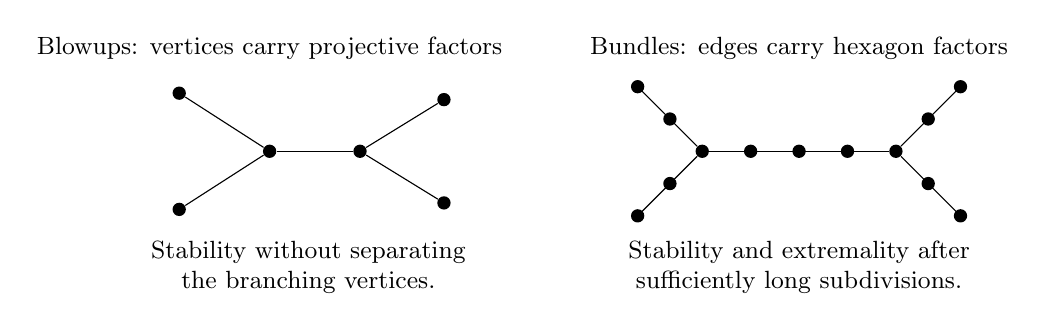
\begin{tikzpicture}[scale=.82,every node/.style={font=\small},
  vertex/.style={circle,fill=black,inner sep=1.7pt}]
\node[align=center] at (0,2.5) {Blowups: vertices carry projective factors};
\node[vertex] (a) at (0,0.9) {};
\foreach \name/\x/\y in {b/-1.4/1.8,c/-1.4/0,d/1.4/0.9}{
 \node[vertex] (\name) at (\x,\y) {}; \draw (a)--(\name);}
\foreach \name/\x/\y in {e/2.7/1.7,f/2.7/0.1}{
 \node[vertex] (\name) at (\x,\y) {}; \draw (d)--(\name);}
\node[align=center,text width=5.7cm] at (.6,-.9)
 {Stability without separating\\
 the branching vertices.};
\begin{scope}[xshift=8.2cm]
\node[align=center] at (0,2.5) {Bundles: edges carry hexagon factors};
\node[vertex] (p) at (-1.5,.9) {};
\node[vertex] (q) at (1.5,.9) {};
\foreach \x in {-.75,0,.75}{\node[vertex] at (\x,.9) {};}
\draw (p)--(q);
\foreach \x/\y in {-2.5/1.9,-2.5/-.1}{
 \draw (p)--(\x,\y);\node[vertex] at (\x,\y) {};
 \node[vertex] at ({(-1.5+\x)/2},{(.9+\y)/2}) {};}
\foreach \x/\y in {2.5/1.9,2.5/-.1}{
 \draw (q)--(\x,\y);\node[vertex] at (\x,\y) {};
 \node[vertex] at ({(1.5+\x)/2},{(.9+\y)/2}) {};}
\node[align=center,text width=5.7cm] at (0,-.9)
 {Stability and extremality after\\
 sufficiently long subdivisions.};
\end{scope}
\end{tikzpicture}
\end{adjustbox}
\caption{Two uses of a subcubic tree. On the left an edge specifies a
codimension-two blowup; on the right it specifies a fibre factor with
opposite twists. The right-hand subdivisions are schematic: the theorem
requires the stated sufficient lengths.}
\label{fig:two-constructions}
\end{figure}
